\begin{minipage}{0.75\linewidth}
\begin{figure}[h]
    \centering
    \begin{adjustbox}{max width=1.0\linewidth, keepaspectratio}
        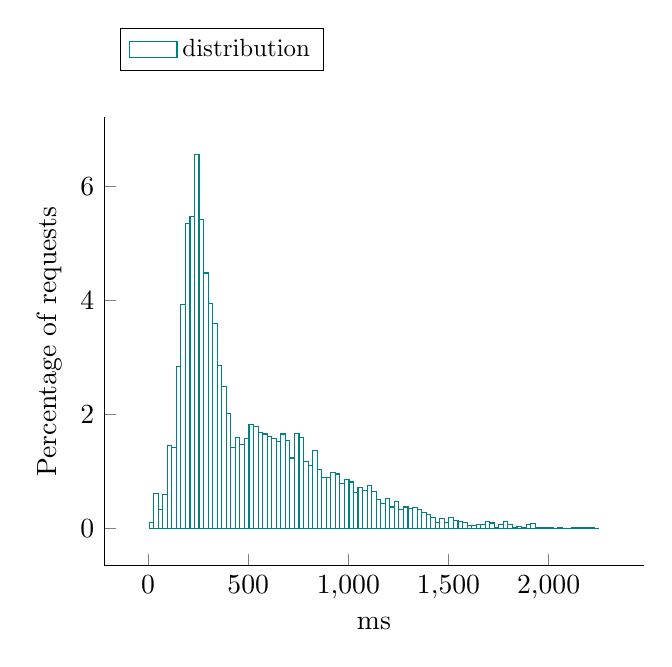
\begin{tikzpicture}
            \begin{axis}[ylabel = Percentage of requests, 
xlabel = ms, 
legend style = {nodes={scale=0.9, transform shape}, at={(0.03,1.2)}, anchor=north west, draw=black, fill=white, align=left, legend columns=3},
area style, mark size = 0pt,
 cycle list name = exotic,
  axis lines* = left]
		\addplot +[ybar interval] coordinates {
			 (5, 0.109375)
			 (27.68, 0.609375)
			 (50.36, 0.328125)
			 (73.04, 0.59375)
			 (95.72, 1.45312)
			 (118.4, 1.42188)
			 (141.08, 2.84375)
			 (163.76, 3.9375)
			 (186.44, 5.35938)
			 (209.12, 5.48438)
			 (231.8, 6.5625)
			 (254.48, 5.42188)
			 (277.16, 4.48438)
			 (299.84, 3.95312)
			 (322.52, 3.59375)
			 (345.2, 2.85938)
			 (367.88, 2.48438)
			 (390.56, 2.01562)
			 (413.24, 1.42188)
			 (435.92, 1.59375)
			 (458.6, 1.46875)
			 (481.28, 1.57812)
			 (503.96, 1.82812)
			 (526.64, 1.78125)
			 (549.32, 1.6875)
			 (572, 1.65625)
			 (594.68, 1.60938)
			 (617.36, 1.57812)
			 (640.04, 1.53125)
			 (662.72, 1.65625)
			 (685.4, 1.54688)
			 (708.08, 1.23438)
			 (730.76, 1.67188)
			 (753.44, 1.59375)
			 (776.12, 1.17188)
			 (798.8, 1.10938)
			 (821.48, 1.35938)
			 (844.16, 1.03125)
			 (866.84, 0.890625)
			 (889.52, 0.890625)
			 (912.2, 0.984375)
			 (934.88, 0.953125)
			 (957.56, 0.78125)
			 (980.24, 0.859375)
			 (1002.92, 0.8125)
			 (1025.6, 0.625)
			 (1048.28, 0.71875)
			 (1070.96, 0.671875)
			 (1093.64, 0.75)
			 (1116.32, 0.640625)
			 (1139, 0.5)
			 (1161.68, 0.4375)
			 (1184.36, 0.53125)
			 (1207.04, 0.375)
			 (1229.72, 0.46875)
			 (1252.4, 0.328125)
			 (1275.08, 0.375)
			 (1297.76, 0.34375)
			 (1320.44, 0.359375)
			 (1343.12, 0.328125)
			 (1365.8, 0.28125)
			 (1388.48, 0.25)
			 (1411.16, 0.1875)
			 (1433.84, 0.109375)
			 (1456.52, 0.171875)
			 (1479.2, 0.109375)
			 (1501.88, 0.1875)
			 (1524.56, 0.140625)
			 (1547.24, 0.125)
			 (1569.92, 0.109375)
			 (1592.6, 0.046875)
			 (1615.28, 0.046875)
			 (1637.96, 0.0625)
			 (1660.64, 0.0625)
			 (1683.32, 0.125)
			 (1706, 0.09375)
			 (1728.68, 0.015625)
			 (1751.36, 0.0625)
			 (1774.04, 0.125)
			 (1796.72, 0.0625)
			 (1819.4, 0.015625)
			 (1842.08, 0.03125)
			 (1864.76, 0.015625)
			 (1887.44, 0.0625)
			 (1910.12, 0.078125)
			 (1932.8, 0.015625)
			 (1955.48, 0.015625)
			 (1978.16, 0.015625)
			 (2000.84, 0.015625)
			 (2023.52, 0)
			 (2046.2, 0.015625)
			 (2068.88, 0)
			 (2091.56, 0)
			 (2114.24, 0.015625)
			 (2136.92, 0.015625)
			 (2159.6, 0.015625)
			 (2182.28, 0.015625)
			 (2204.96, 0.015625)
			 (2227.64, 0)
			 (2250.32, 0)
		};
\addlegendentry{distribution};
           \end{axis}
      \end{tikzpicture}
  \end{adjustbox}
  \caption{Response time distribution - req = ReadTimeline-0}
\end{figure}
\end{minipage}\hfill\begin{minipage}{0.18\linewidth}
\begin{table}[h]
\begin{tabular}{|cc|}
\hline
\textbf{} & \textbf{ms}\\ \hline
 \Xhline{0.005\arrayrulewidth}
min & 5\\
 \Xhline{0.005\arrayrulewidth}
max & 2273\\
 \Xhline{0.005\arrayrulewidth}
mean & 512\\
 \Xhline{0.005\arrayrulewidth}
std & 356\\
\hline
\hline
 \Xhline{0.005\arrayrulewidth}
25th & 241\\
 \Xhline{0.005\arrayrulewidth}
50th & 376\\
 \Xhline{0.005\arrayrulewidth}
75th & 717\\
 \Xhline{0.005\arrayrulewidth}
80th & 797\\
 \Xhline{0.005\arrayrulewidth}
85th & 905\\
 \Xhline{0.005\arrayrulewidth}
90th & 1035\\
 \Xhline{0.005\arrayrulewidth}
95th & 1228\\
 \Xhline{0.005\arrayrulewidth}
99th & 1634\\
\hline
\end{tabular}
\caption{Response time}
\end{table}
\end{minipage}\hfill